\documentclass[10pt,letterpaper]{article} 
\usepackage{tikz}
\usepackage{tools}
\usepackage{enumitem}
\usepackage{listings}
\usepackage{hyperref}
\usepackage{algorithm}
\usepackage{algorithmic}
\usepackage{tcolorbox}
\definecolor{gray}{RGB}{220,220,220}
%\usepackage{framed}
\newcommand{\code}[1]{
\colorbox{gray}{\texttt{#1}}
}
%\definecolor{shadecolor}{gray}
\lstset{language=Python}
%\lstset{frame=lines}
%\lstset{caption={Insert code directly in your document}}
\lstset{label={lst:code_direct}}
\lstset{basicstyle=\footnotesize}

%\usepackage{graphicx}‎‎
%\usefonttheme{serif}‎
%\usepackage{ptext}‎
%\usepackage{xepersian}
%\settextfont{B Nazanin}
\usepackage{lipsum}
\setlength{\parindent}{0pt}
\setlength{\parskip}{1em}
\newcommand{\pf}{$\blacksquare$}

\newcommand{\Span}{\text{Span}}
\newcommand{\NF}{\text{NF}}
\newcommand{\EDFA}{\text{EDFA}}
\newcommand{\ASE}{\text{ASE}}

\newcommand{\bns}{\textit{broadcast-and-select}  architecture}
\newcommand{\Bns}{\textit{Broadcast-and-select} architecture}

\newcommand{\rns}{\textit{route-and-select} architecture}
\newcommand{\Rns}{\textit{Route-and-select} architecture}

\newcommand{\red}[1]{{\color{red}#1}}

\newcounter{QuestionNumber}
\setcounter{QuestionNumber}{1}

\newcommand{\Q}{
\textbf{Question \theQuestionNumber)}
\stepcounter{QuestionNumber}
}
\newcommand{\EX}{\Bbb E}
\newcommand{\nl}{\newline\newline}
%\newcommand{\pic}[2]{
%\begin{center}
%\includegraphics[width=#2]{#1}
%\end{center}
%}
\begin{document}
\large
\begin{center}
In the name of beauty

The $3^\text{rd}$ simulation assignment of Optical Networks course
\hl
\end{center}
\section{Foreword}
In this simulation problem set, we aim at implementing the Dijkstra algorithm, a greedy heuristic that finds the shortest path between two nodes of a graph when each link of a graph is assigned a metric and the total path matric is the sum of the metrics of links comprising that path. Our programming language is Python. In the following, we will walk through the steps of Dijkstra algorithm and test cases for it.

\section{Problem Framework}
Any graph consisting of nodes and links, has an adjacency matrix. Labeling the nodes of the graph with $N$ nodes from $0$ to $N-1$, the adjacency matrix is an $N\times N$ matrix with  the following definition of its entries $m_{ij}$:
\begin{equation}
m_{ij}=
%\begin{cases}
\text{link metric from node $i-1$ to node $j-1$}
%\end{cases}
\end{equation}
where $i,j\in \{1,2,\cdots,N\}$ and $m_{ij}$ denotes the entry of the $i$th row and $jth$ column of the adjacency matrix. A weighted graph is simple\footnote{A simple weighted graph is defined as that with bidirectional links whose metrics are equal at both directions.} if and only if $m_{ij}=m_{ji}$. We also agree to write $m_{ii}=0$. Two graph topologies with their adjacency matrix are illustrated in figure \ref{fig:ex}. The steps of Dijkstra algorithm are as mentioned in algorithm \ref{alg:dij}.

\begin{algorithm}[h]
\caption{Dijkstra algorithm for graph with non-negative link metrics}
\textbf{Input:}
Adjacency matrix of a graph $M_{N\times N}$, source index $s$, destination index $d$

\textbf{Output:}
A list $l$ of consecutive nodes representing the shortest path from source to destination

\textbf{Initialization:}

Create a list of floats where the $i$th entry is the distance of source to the $i$th node if it is a neighbor of source and $10^{10}$ otherwise; call this vector $D$

Create a list of nodes where the $i$th entry is equal to $s$; call this vector $P$
\begin{algorithmic}
\STATE F=$\{s\}$
\WHILE{$F\ne \{0,1,2,\cdots,N-1\}$}
\STATE Find $i$ such that $D_i$ is minimum in $D$
\STATE Add $i$ to $F$
\FOR{all graph nodes $j$ not in $F$}
\IF{$D_i+m_{ij}<D_j$}
\STATE $D_j\longleftarrow D_i+m_{ij}$
\STATE $P_j\longleftarrow i$
\ENDIF
\ENDFOR
\ENDWHILE
\end{algorithmic}
\label{alg:dij}
\end{algorithm}
\newpage
\begin{figure}[htbp]
\centering
%%%%%%%%%%%%%%%%%%%%%%%%%%%%
\begin{subfigure}{0.49\textwidth}
\centering
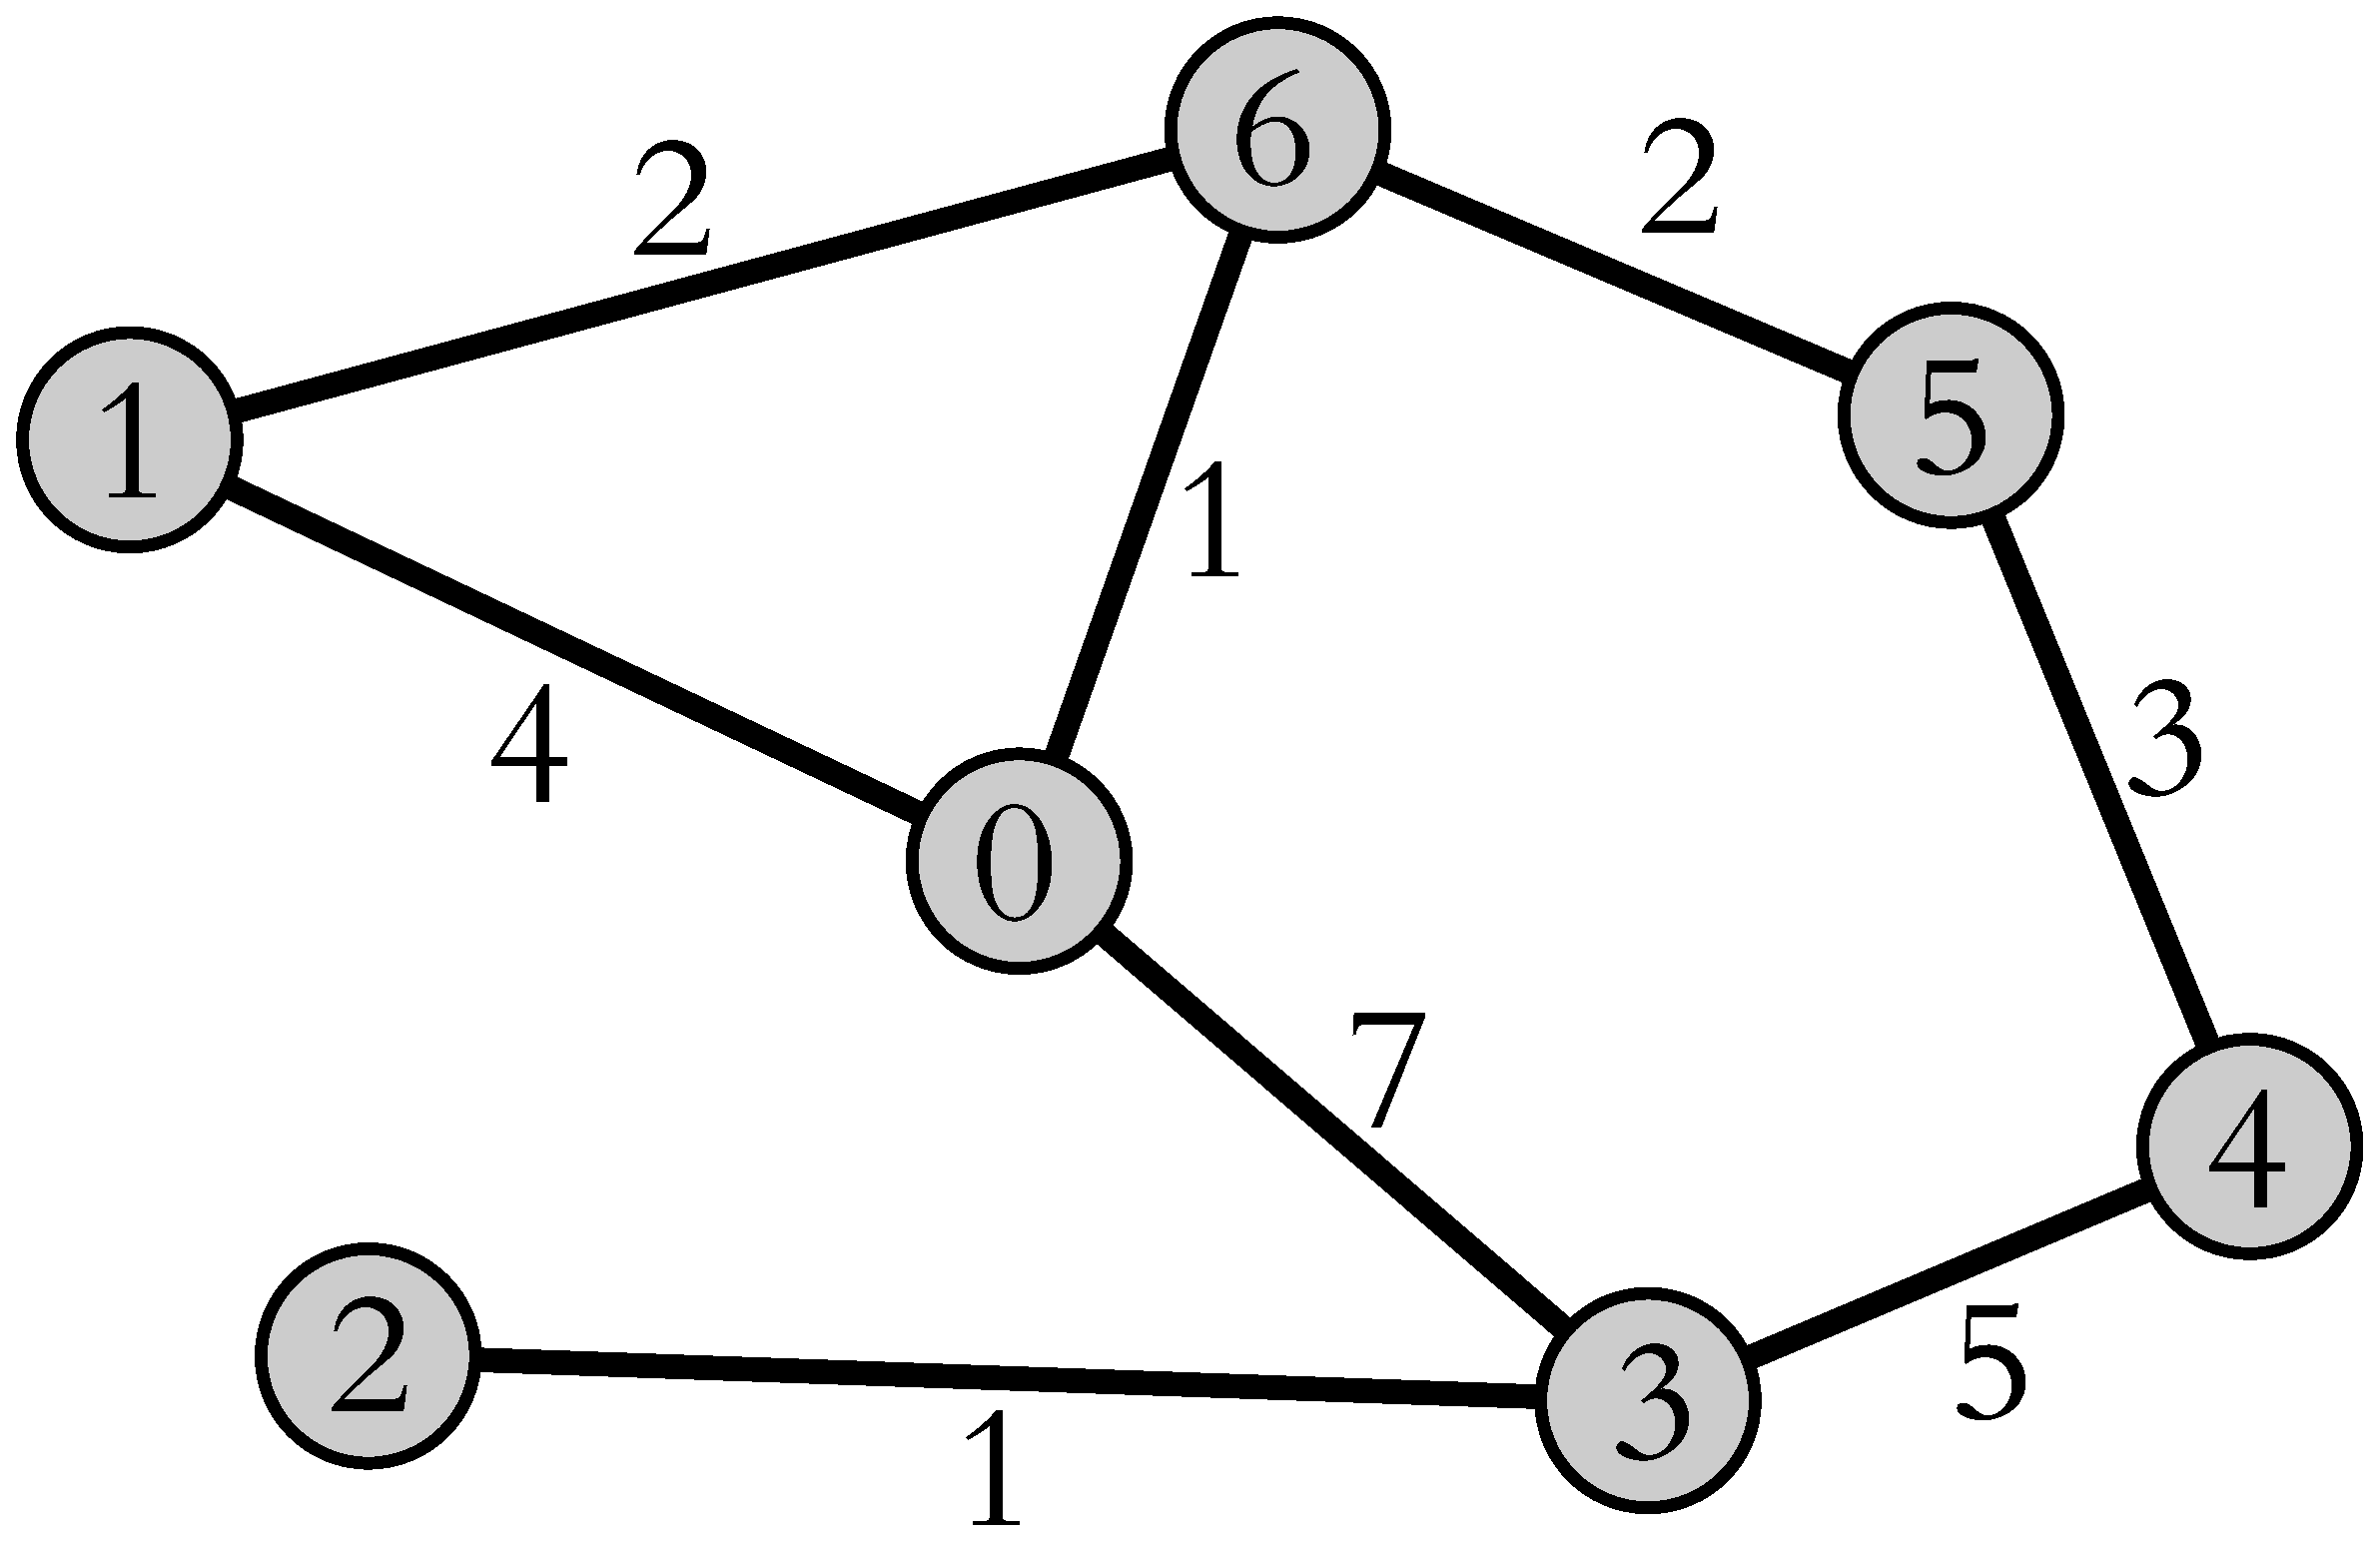
\includegraphics[width=50mm]{dij1.eps}
\end{subfigure}
%%%%%%%%%%%%%%%%%%%%%%%%%%%%
\begin{subfigure}{0.49\textwidth}
{
\Large
$
M=\begin{bmatrix}
0&4&\infty&7&\infty&\infty&1\\
4&0&\infty&\infty&\infty&\infty&2\\
\infty&\infty&0&1&\infty&\infty&\infty\\
7&\infty&1&0&5&\infty&\infty\\
\infty&\infty&\infty&5&0&3&\infty\\
\infty&\infty&\infty&\infty&3&0&2\\
1&2&\infty&\infty&\infty&2&0
\end{bmatrix}
$
}
\end{subfigure}
%%%%%%%%%%%%%%%%%%%%%%%%%%%%
\vspace{10mm}
\begin{subfigure}{0.49\textwidth}
\centering
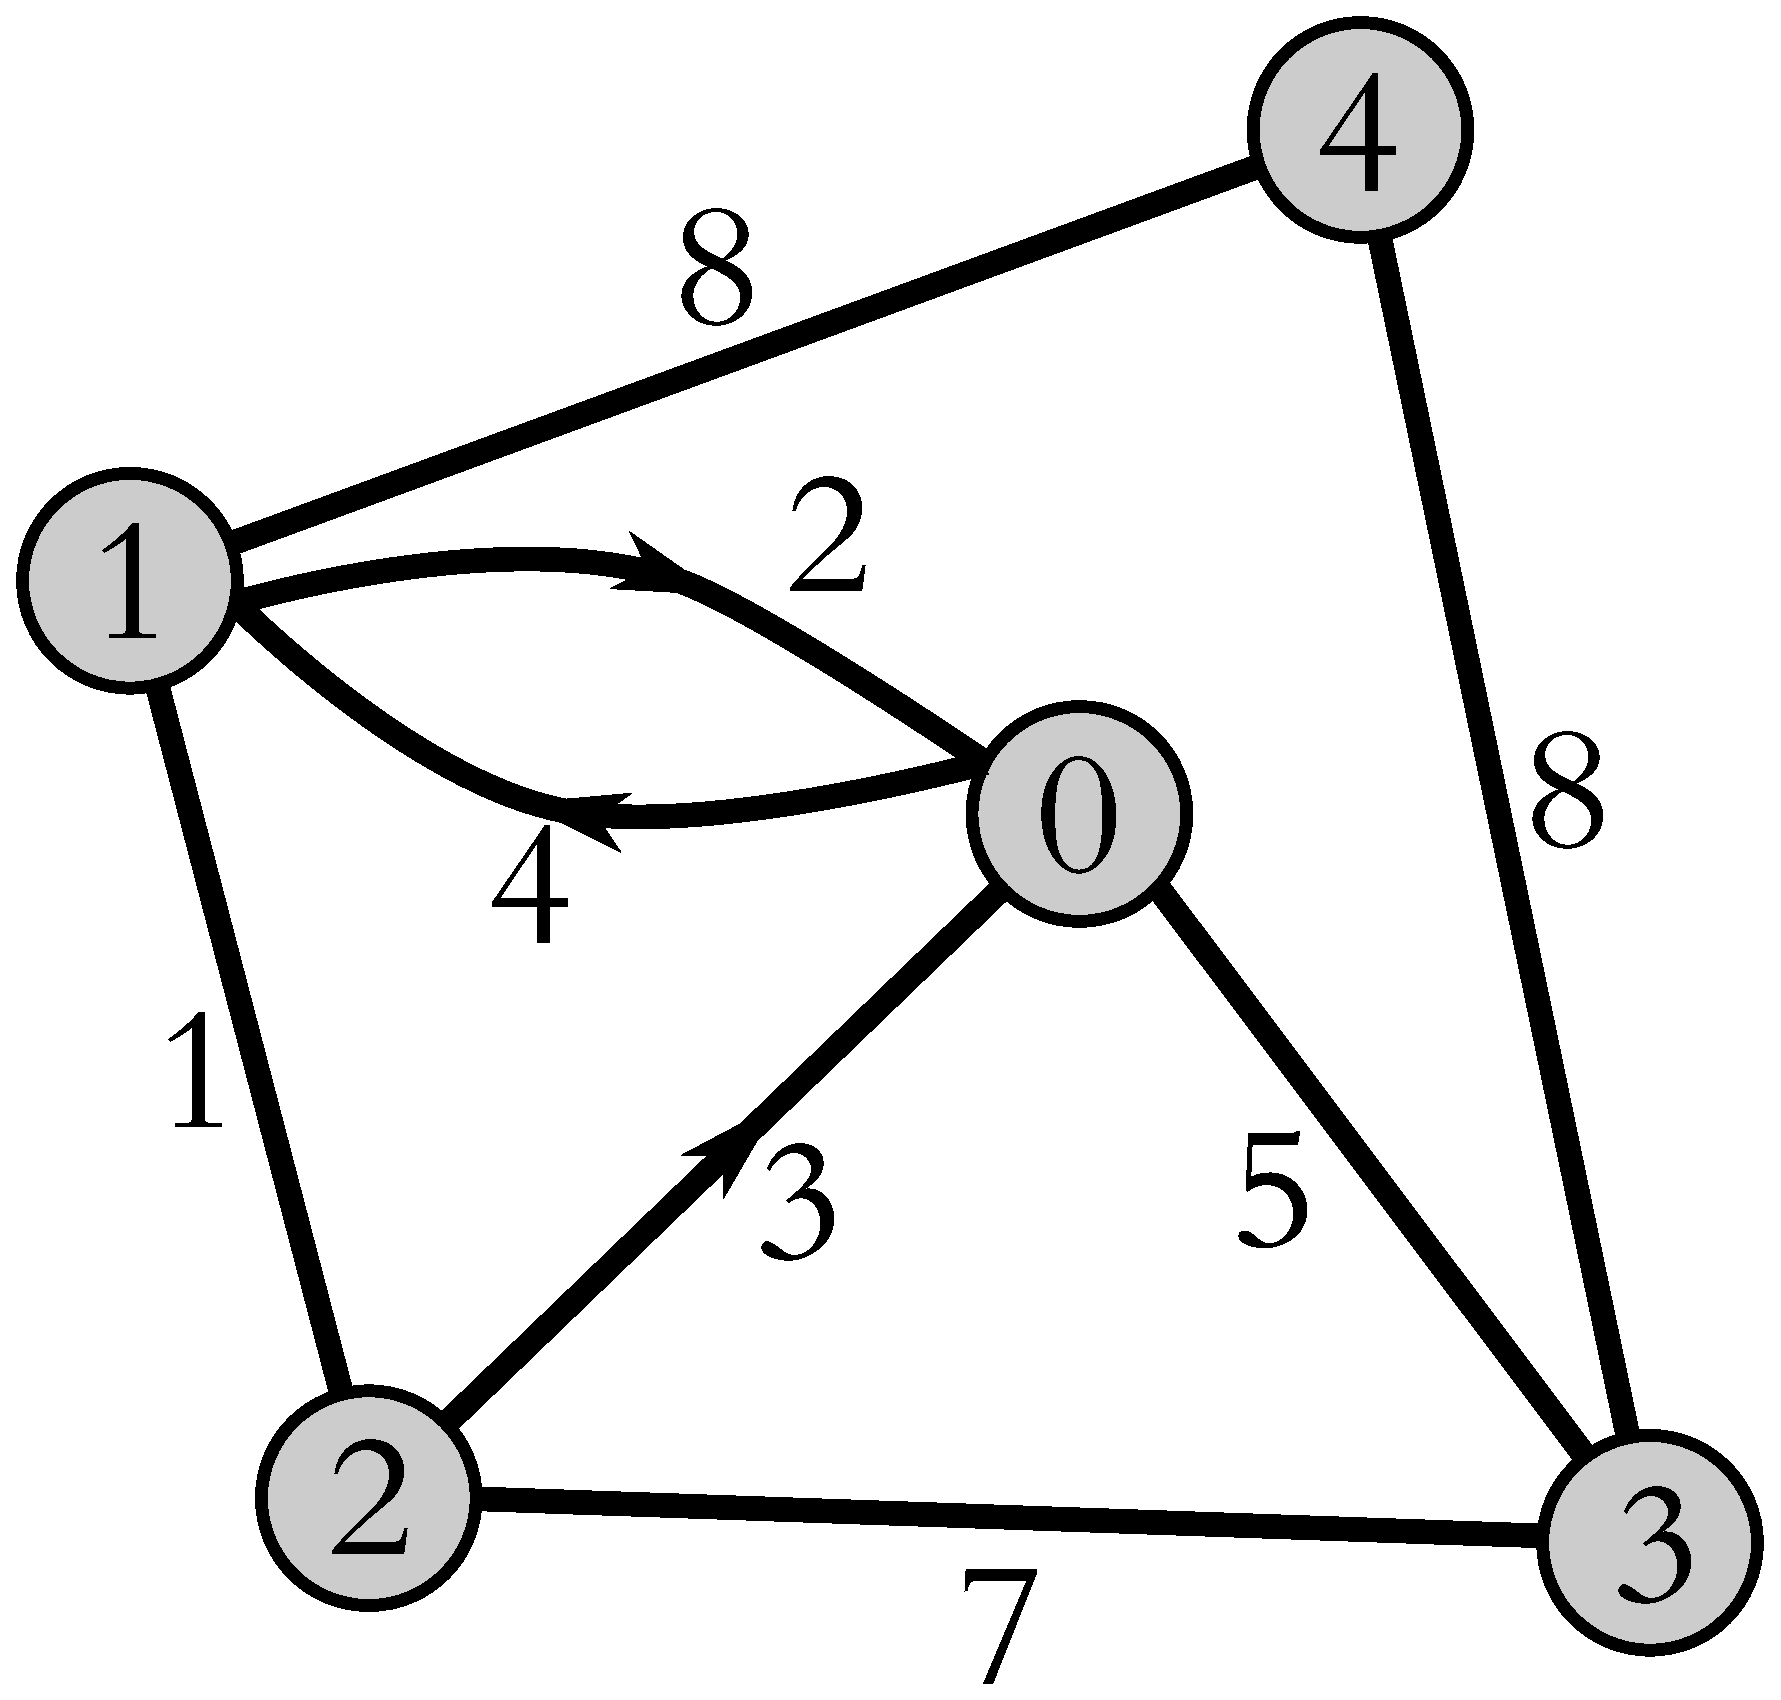
\includegraphics[width=40mm]{dij2.eps}
\end{subfigure}
%%%%%%%%%%%%%%%%%%%%%%%%%%%%
\begin{subfigure}{0.49\textwidth}
{
\Large
$
M=\begin{bmatrix}
0&4&\infty&5&\infty\\
2&0&1&\infty&8\\
3&1&0&7&\infty\\
5&\infty&7&0&8\\
\infty&8&\infty&8&0\\
\end{bmatrix}
$
}
\end{subfigure}
%%%%%%%%%%%%%%%%%%%%%%%%%%%%
\caption{Two examples of graph topologies with their corresponding adjacency matrices; (a) simple graph with symmetric adjacency matrix and (b) directed graph with asymmetric adjacency matrix}
\label{fig:ex}
\end{figure}

\section{Implementation}

You are expected to write a function that takes the adjacency matrix of a generally directed graph, source index and destination index and yields the sequence of consecutive nodes from source to destination. This function must use the Dijkstra algorithm at its core. For example, if the function is named \texttt{ShortestPath}, the header and structure of the function would be

\texttt{\ \ \ \ def ShortestPath(AdjMat,s,d):}

\texttt{\ \ \ \ $\qquad$\# Function structure which uses Dijkstra algorithm}

\texttt{\ \ \ \ $\qquad$return ListofNodes}

Sample of input and output:

\texttt{\ \ \ \ AdjMat=[[0,2,1,1e6], [2,0,1,3], [1,1,0,1], [1e6,3,1,0]]}

\texttt{\ \ \ \ s=1, d=3}

\texttt{\ \ \ \ print(ShortestPath(AdjMat,s,d)) \# prints [1, 2, 3]}

Note that for nodes $i$ and $j$ with no direct link between them, $m_{ij}$ is equal to $\infty$. Since $\infty$ is undefined by Python, we substitute $\infty$ with a large enough float like $10^6$, as we did in the example above.

You should hand in the code you have written for function \texttt{ShortestPath}. Four tests would be applied to your function and your grade would be determined by the number of tests your function passes.

\end{document}